\section{MedWorld-JEPA}
\label{sec:method}

% Introduce the overall method before the detailed state construction.
\begin{figure*}[t]
    \centering
    % User-selected Figure 1: ppt/ppt/fig1_v8.pptx with the obsolete stage label removed (2026-09-19).
    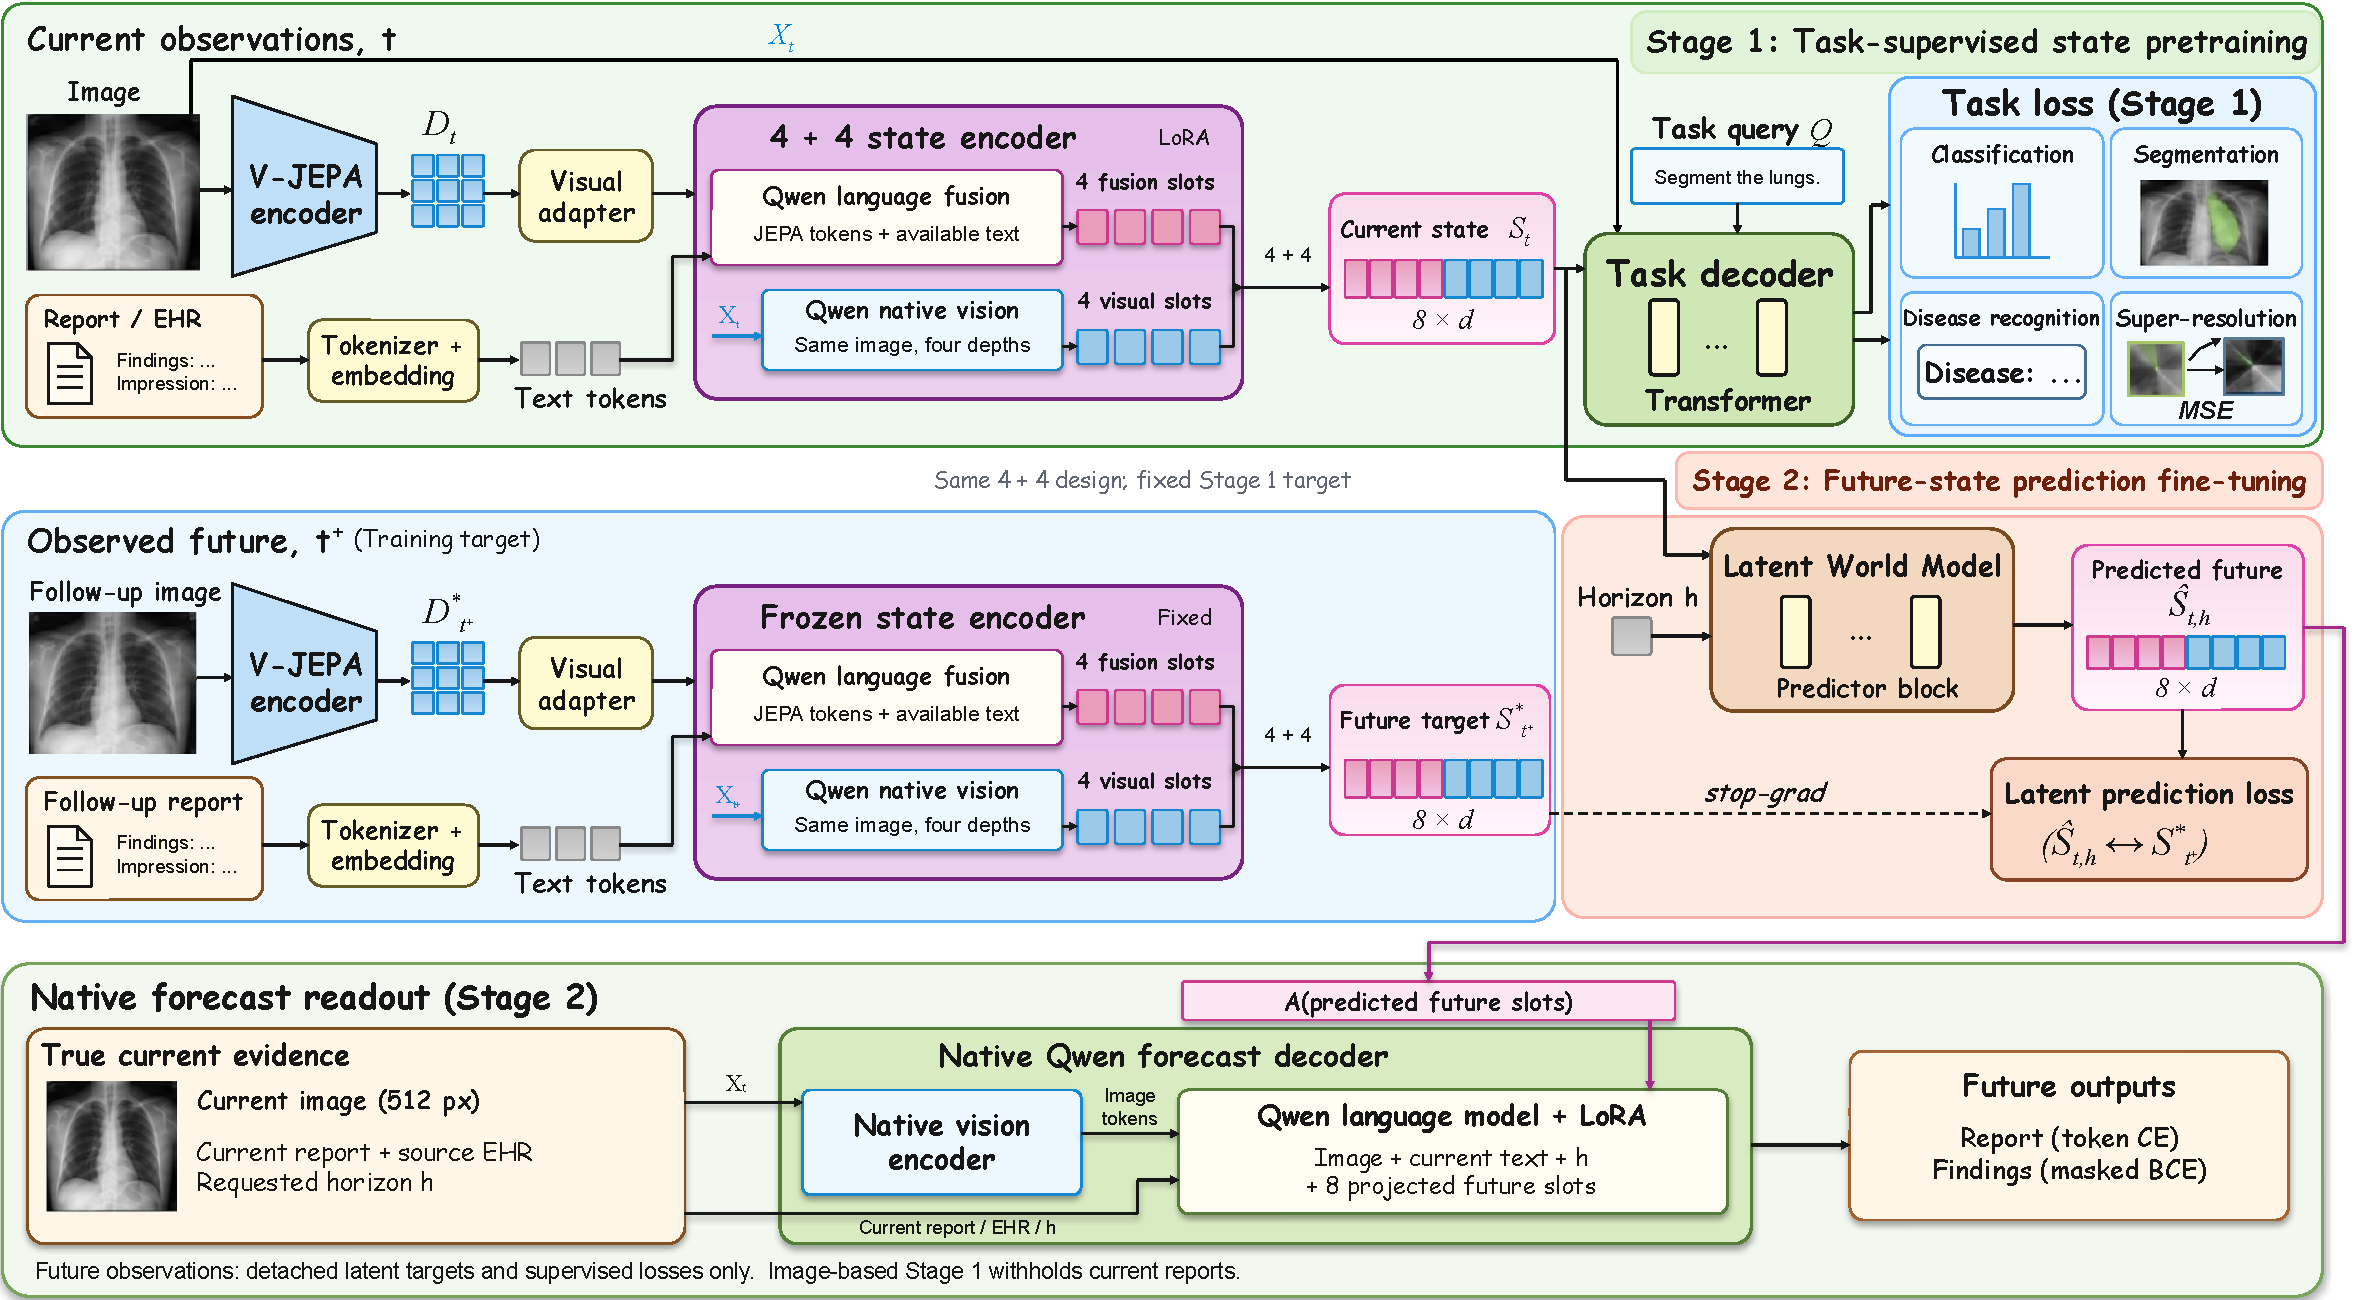
\includegraphics[width=\textwidth]{ppt/ppt/fig1_v8.pdf}
    \caption{Overview of \method{}. The state $S\in\mathbb R^{8\times d}$ supports task decoding and horizon-conditioned prediction; Figure~\ref{fig:task_supervised_slots} details its construction. The current task decoder combines native image tokens with all eight slots for classification, VQA, and segmentation. The world model maps $(S_t,h)$ to $\widehat S_{t,h}$, supervised by the stop-gradient follow-up target $S^*_{t^+}$. Task supervision and latent temporal prediction are optimized jointly from the first update. \pending{update the schematic task examples and image-token pathway to match the three-task readout in \cref{eq:task_interface}}. The encoding blocks are schematic; the multi-depth readouts are specified in Figure~\ref{fig:task_supervised_slots}.}
    \label{fig:medworld_jepa_overview}
\end{figure*}

\subsection{Task Definition}
\label{sec:formulation}

We study medical state representation and future state prediction from longitudinal observations. At time $\tau$, an observation is $O_\tau=(X_\tau,C_\tau;m_\tau)$, where $X_\tau$ is a medical image, $C_\tau$ is its report or other admissible clinical text, and $m_\tau\in\{0,1\}^2$ records modality availability. We consider image-bearing observations, with clinical text when available. Our primary setting uses an image--report pair at both the current time $t$ and an observed follow-up $t^+>t$.

An encoder $E_\eta$ maps each observation to multimodal state tokens $S_\tau\in\mathbb R^{K\times d}$. Tasks requiring spatial detail additionally receive the input image $X_\tau$ directly. Given $S_t$ and a requested temporal horizon $h$, a latent world model predicts the follow-up state:
\begin{equation}
    \begin{gathered}
        O_t \xrightarrow{\ E_\eta\ } S_t,\\
        (S_t,h) \xrightarrow{\ P_\psi\ } \widehat S_{t,h}
        \approx S^*_{t^+}.
    \end{gathered}
    \label{eq:future_prediction}
\end{equation}
The target $S^*_{t^+}$ is encoded from the actual follow-up. We distinguish the requested horizon $h$ from the realized follow-up time $t^+$; their association is set by the temporal sampling protocol. The retrospective forecasting protocol assumes the current report is available at the source observation; other clinical records must satisfy the source-time cutoff. Follow-up images and text enter the target branch.

The model has two objectives: \emph{predict future states} at a specified horizon and \emph{learn reusable states} for classification, visual question answering, report generation, phrase grounding, segmentation, and super-resolution. State construction precedes both the task request and the horizon condition. A state represents the available medical observations, without assuming access to all variables governing a patient's course. Prediction concerns observational follow-ups and carries no treatment-intervention semantics.


\subsection{State Representation}
\label{sec:state_representation}

\paragraph{Slot-based multimodal representation.}
We encode each medical observation as a compact set of state slots that combines vision--language and visual information across multiple network depths. This representation brings clinical semantics and spatial evidence into a common latent space for downstream understanding and temporal prediction.

Given an observation $O_\tau$, the vision--language branch integrates adapted features from a frozen JEPA encoder with the available report, while the VLM's native vision encoder provides visual features before language fusion. We select four approximately evenly spaced depths from each branch to capture information at different levels of abstraction. Four learned query tokens summarize the vision--language sequence, with each query read out at its corresponding selected depth. In the visual branch, a learned query pools the projected patch features at each selected depth. The resulting slots are projected to a common width and concatenated:
\begin{equation}
    \begin{aligned}
        s_{\tau,j}^{f}
        &=r_j^{f}\!\left(H_\tau^{(\ell_j)}\right),\qquad
        s_{\tau,j}^{v}
        =r_j^{v}\!\left(F_\tau^{(k_j)}\right),\\
        S_\tau
        &=\left[S_\tau^{f};S_\tau^{v}\right]
        \in\mathbb{R}^{8\times d},
    \end{aligned}
    \label{eq:vlm_state}
\end{equation}
where $j=1,\ldots,4$, $d=1024$, and $r_j^{f}$ and $r_j^{v}$ denote the source-specific readouts. The four vision--language slots and four visual slots retain a fixed ordering by source and depth, yielding a structured representation of the observation.

The state is constructed independently of the downstream query and prediction horizon, allowing the same observation representation to support different tasks and temporal predictions. For downstream understanding, a shared Transformer decoder combines all eight slots with native image tokens, and its image-token outputs feed the classification, VQA, and segmentation heads. The slots contribute observation-level context alongside direct spatial evidence from the image. Task supervision jointly optimizes the slot readouts and adapted feature sources, encouraging the learned representation to retain information relevant to clinical and spatial understanding.

\paragraph{Visual Slot Spatial Consistency (VSSC).}
Compressing an observation into a small number of slots can discard local visual structure. We introduce VSSC to explicitly encourage fine-grained spatial information to remain recoverable from the four visual slots. An auxiliary reconstruction module uses spatial coordinate queries to attend to $S_\tau^{v}$, producing a dense feature field through interpolation and convolutional refinement. Its sample-specific information comes entirely from the visual slots.

We supervise this field using a frozen, unadapted copy of the native vision encoder. The teacher independently encodes the original image and two cropped views, providing spatial feature targets through a fixed projection. For each view, the reconstructed field undergoes the corresponding spatial transformation and average downsampling before comparison with the teacher:
\begin{equation}
    \begin{aligned}
        \mathcal L_{\mathrm{VSSC}}
        =\frac{1}{3}\sum_{a=0}^{2}\ell_{\Omega_a}\Bigl(
        &\mathcal A_a\!\left(G_\xi(S_\tau^{v})\right),\\
        &\operatorname{sg}\!\left[\Phi_0(T_a(X_\tau))\right]\Bigr).
    \end{aligned}
    \label{eq:vssc_loss}
\end{equation}
Here, $G_\xi$ is the reconstruction module, $\Phi_0$ is the frozen teacher with its fixed projection, and $T_a$ denotes the identity view or a crop transformation. The operator $\mathcal A_a$ applies the corresponding transformation and downsampling to the reconstructed field. The loss $\ell_{\Omega_a}$ measures mean squared distance between channel-normalized feature vectors over valid spatial locations $\Omega_a$.

Matching independently encoded views encourages the slots to retain local information that remains spatially consistent under changes in view. VSSC updates the visual-slot pathway and auxiliary reconstruction module during segmentation training. The reconstruction module and teacher are used only during training, leaving the downstream inference architecture unchanged.

\subsection{State Prediction}
\label{sec:state_prediction}

\paragraph{Horizon-conditioned state dynamics.}
Building on the multimodal representation in Sec.~\ref{sec:state_representation}, we model patient evolution as a transition between observation states in latent space. Given the current state $S_t=E_\eta(O_t)$ and a requested time interval $h$, a predictor estimates the state of a follow-up examination:
\begin{equation}
    \widehat S_{t,h}
    =P_\psi(S_t,h)
    \in\mathbb{R}^{8\times d}.
    \label{eq:state_transition}
\end{equation}
The predictor jointly processes all eight slots, allowing temporal modeling to incorporate both vision--language and visual information. A learned time embedding encodes the sign and log-magnitude of the interval, accommodating irregular examination times and directed observation pairs. A Transformer combines this embedding with the state slots and predicts a residual update to the normalized source state. Slot ordering is preserved throughout prediction, maintaining correspondence between feature sources and representation depths. Each requested horizon is predicted directly from the current state; the observation encoder remains independent of the time condition.

\paragraph{Joint-embedding predictive learning.}
We adopt a JEPA-style objective that learns temporal dynamics by predicting the representation of an actual follow-up examination. The follow-up image and report are encoded by a target encoder with the same state-construction architecture:
\begin{equation}
    S_{t^+}^{*}=E_{\bar\eta}(O_{t^+}),
    \qquad h=t^+-t.
    \label{eq:followup_target}
\end{equation}
The target encoder follows an exponential moving average of the online encoder. We align the predicted and target states using a normalized latent prediction loss:
\begin{equation}
    \mathcal L_{\mathrm{future}}
    =\frac{1}{8d}
    \left\|
    \mathcal N(\widehat S_{t,h})
    -\operatorname{sg}\!\left[\mathcal N(S_{t^+}^{*})\right]
    \right\|_F^2,
    \label{eq:future_latent_loss}
\end{equation}
where $\mathcal N$ applies non-affine LayerNorm independently to each slot and $\operatorname{sg}$ denotes stop-gradient. The objective updates both the predictor and the trainable current-state encoder, allowing the demands of longitudinal prediction to shape the medical representation itself. Follow-up images and reports enter only the target branch during training. At inference, the current observation and requested interval determine the predicted follow-up state.

% Place the compact slot detail near the training discussion, after the
% state construction and dynamics text, to separate it from Figure 1.
\begin{figure*}[t]
    \centering
    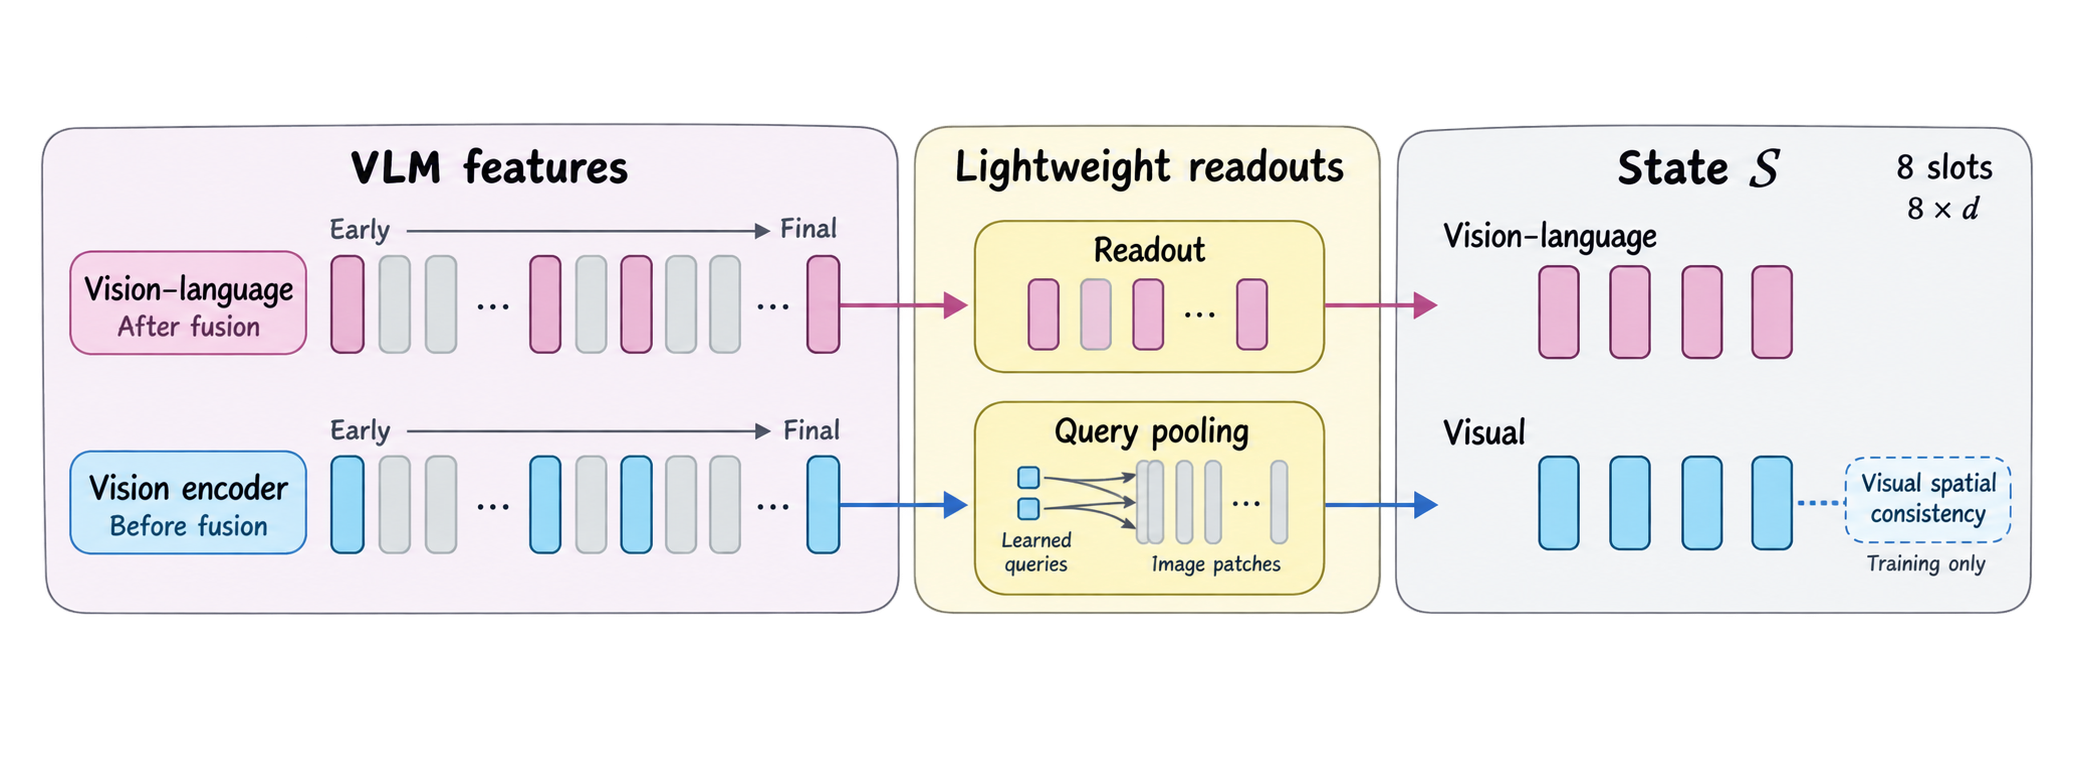
\includegraphics[width=\textwidth]{ppt/source/fig2_v4.png}
    \caption{Construction of the eight state slots. Lightweight readouts extract four vision--language slots and four visual slots from one early, two intermediate, and the final layer of their respective feature sources. Visual slots use only pre-fusion vision features and optionally receive training-only spatial consistency supervision.}
    \label{fig:task_supervised_slots}
\end{figure*}

\subsection{Single-Stage Joint Training}
\label{sec:training}

Single-time-point annotations supervise state content, while longitudinal pairs supervise its evolution. We optimize both in one continuous training run from pretrained JEPA and VLM weights. Every optimizer update combines a current-task batch with a temporal batch, jointly training the online state encoder, dynamics predictor, and active task heads.

\paragraph{Current-task supervision.}
Starting from pretrained JEPA and VLM weights, we jointly train the adapters, multi-scale slot readouts, task decoders, and selected VLM parameters using parameter-efficient adaptation~\citep{hu2022lora}; JEPA remains frozen. The current-task component cycles through classification, segmentation, and VQA, drawing each batch from its task-specific training pool. Each task contributes once every three optimizer updates, alongside temporal supervision at every update. The task objective is
\begin{equation}
    \mathcal L_{\mathrm{task}}
    =\frac{1}{3}\sum_{q\in\mathcal Q}
      \mathbb E_{i\sim\mathcal D_q}
      \left[\ell_q\!\left(\widehat y_i^{(q)},y_i^{(q)}\right)\right],
    \label{eq:task_loss}
\end{equation}
where $\mathcal Q$ contains the three tasks and $\mathcal D_q$ is the corresponding training pool. Each task combines native image tokens $I_\tau$ with the state through a shared Transformer decoder:
\begin{equation}
    \begin{aligned}
        Z_\tau &= T_\omega\bigl([\pi_I(I_\tau);\pi_S(S_\tau)]\bigr)_{1:N_I},\\
        \widehat y_\tau^{(q)} &= H_{\omega_q}(Z_\tau,Q_q).
    \end{aligned}
    \label{eq:task_interface}
\end{equation}
Here $\pi_I$ and $\pi_S$ project image tokens and slots to a common width; $H_{\omega_q}$ is the task-specific head. The VQA question enters only the task readout. Classification uses class-weighted binary cross-entropy with unknown and uncertain labels masked, VQA uses token cross-entropy, and segmentation uses Dice and pixelwise binary cross-entropy.

There is no stop-gradient between the task decoders and slot readouts. Task gradients flow through $S$ into the learned aggregation/projection modules and any adapted source layers, jointly with decoder updates. All three tasks supervise both slot groups through the shared task decoder. Thus training updates the shared parameters that produce observation-dependent slots, rather than treating each sample's slots as independent optimization variables. Current-task inputs withhold the same-exam report. Encoder and VQA-decoder LoRA parameters are independent, while immutable pretrained language weights share storage.

\paragraph{Joint objective.}
Every optimizer update combines a current-task batch with directed same-patient observation pairs, primarily from MIMIC-CXR~\citep{johnson2019mimiccxr}. The expected objective is
\begin{equation}
    \mathcal L_{\mathrm{joint}}
    =\lambda_S\mathcal L_{\mathrm{future}}+\mathcal L_{\mathrm{task}}
     +\lambda_V\mathcal L_{\mathrm{VSSC}},
    \label{eq:joint_loss}
\end{equation}
where $\lambda_S=1$ and $\lambda_V=0.1$ when visual consistency is enabled. The consistency term is zero outside segmentation updates; its expectation follows the same three-task cycle. The latent loss updates the predictor and source-state encoder, while the task loss updates the shared decoder, active task head, and its input pathways. There are no future-report or future-finding losses in this implementation. JEPA remains frozen. Temporal prediction and downstream task performance require separate held-out evaluations.

\paragraph{Target updates and implementation choices.}
At model initialization, the target encoder copies the online encoder, including all trainable state-construction parameters. The target forward pass uses evaluation mode and stop-gradient. After every joint optimizer update, its parameters follow an exponential moving average:
\begin{equation}
    \bar\eta\leftarrow m\bar\eta+(1-m)\eta,\qquad m=0.99.
    \label{eq:target_ema}
\end{equation}
EMA covers all trainable state-encoder parameters, including LoRA, the JEPA adapter, slot queries, positional embeddings, and readouts; it excludes the predictor and task decoders. Immutable pretrained parameters remain frozen and can share storage, while target buffers are copied from the online encoder. Joint training uses AdamW with learning rates $5\times10^{-5}$ for LoRA and $10^{-4}$ for other trainable parameters, weight decay 0.01, and gradient clipping at norm 1. One optimizer is retained throughout the run. LoRA has rank 8 and scaling factor $16/8$, and is applied at the four selected language and vision depths. Distributed training synchronizes gradients across ranks before the optimizer and EMA updates.

\paragraph{Data separation.}
Current-task and temporal batches use fixed data manifests with a global patient-level holdout across current tasks and temporal pairs. Conflicting records are removed from lower-priority splits, preserving test over validation over training membership. Current-task supervision uses MIMIC-CXR finding labels, fixed CXAS segmentation targets, and MIMIC-CXR-VQA question--answer pairs; Montgomery supplies an external human-mask test set. Temporal inputs consist of source images and reports with signed actual time intervals. MIMIC-IV contributes the existing admission linkage, but laboratory results, medications, and vital signs are not model inputs. Evaluation predicts from source observations before accessing target references.
